%%%%%%%%%%%%%%%%%%%%%%%%%%%%%%%%%%%%%%%%%%%%%%%%%%%%%%%%%%%%%%%%%%%%
%% I, the copyright holder of this work, release this work into the
%% public domain. This applies worldwide. In some countries this may
%% not be legally possible; if so: I grant anyone the right to use
%% this work for any purpose, without any conditions, unless such
%% conditions are required by law.
%%%%%%%%%%%%%%%%%%%%%%%%%%%%%%%%%%%%%%%%%%%%%%%%%%%%%%%%%%%%%%%%%%%%

\documentclass[
  digital, %% This option enables the default options for the
           %% digital version of a document. Replace with `printed`
           %% to enable the default options for the printed version
           %% of a document.
  oneside, %% This option enables double-sided typesetting. Use at
           %% least 120 g/m² paper to prevent show-through. Replace
           %% with `oneside` to use one-sided typesetting; use only
           %% if you don’t have access to a double-sided printer,
           %% or if one-sided typesetting is a formal requirement
           %% at your faculty.
  table,   %% This option causes the coloring of tables. Replace
           %% with `notable` to restore plain LaTeX tables.
  lof,     %% This option prints the List of Figures. Replace with
           %% `nolof` to hide the List of Figures.
  lot,     %% This option prints the List of Tables. Replace with
           %% `nolot` to hide the List of Tables.
  %% More options are listed in the user guide at
  %% <http://mirrors.ctan.org/macros/latex/contrib/fithesis/guide/mu/fi.pdf>.
]{fithesis3}
%% The following section sets up the locales used in the thesis.
\usepackage[resetfonts]{cmap} %% We need to load the T2A font encoding
\usepackage[T1,T2A]{fontenc}  %% to use the Cyrillic fonts with Russian texts.
\usepackage[
  main=english, %% By using `czech` or `slovak` as the main locale
                %% instead of `english`, you can typeset the thesis
                %% in either Czech or Slovak, respectively.
  english, german, russian, czech, slovak %% The additional keys allow
]{babel}        %% foreign texts to be typeset as follows:
%%
%%   \begin{otherlanguage}{german}  ... \end{otherlanguage}
%%   \begin{otherlanguage}{russian} ... \end{otherlanguage}
%%   \begin{otherlanguage}{czech}   ... \end{otherlanguage}
%%   \begin{otherlanguage}{slovak}  ... \end{otherlanguage}
%%
%% For non-Latin scripts, it may be necessary to load additional
%% fonts:
\usepackage{paratype}
\def\textrussian#1{{\usefont{T2A}{PTSerif-TLF}{m}{rm}#1}}
%%
%% The following section sets up the metadata of the thesis.
\thesissetup{
    date          = \the\year/\the\month/\the\day,
    university    = mu,
    faculty       = fi,
    type          = bc,
    author        = Marek Mravík,
    gender        = m,
    advisor       = RNDr. Lukáš Němec,
    title         = {Virtual assistant},
    TeXtitle      = {Virtual assistant},
    keywords      = {virtual, assistant, AI, speech recognition, text                 to speech, machine learning, deep learning, Amazon, Alexa, Google, Apple, Siri},
    TeXkeywords   = {virtual, assistant, AI, speech recognition, text                 to speech, machine learning, deep learning, Amazon, Alexa, Google, Apple, Siri},
    abstract      = {This thesis is focused on virtual assistants, their history, availability and comparison. For purpose of this thesis I have selected Amazon Alexa, Google Assistant and Apple Siri. Security, speech-to-text understanding and functionality of these assistants will be analyzed and tested. Second part of the thesis defines how a virtual assistant should work, behave and be designed at my opinion and a really simple basic assistant with few functions is implemented.},
    thanks        = {These are the acknowledgements for my thesis, which can

                     span multiple paragraphs.},
    bib           = example.bib,
}
\usepackage{makeidx}      %% The `makeidx` package contains
\makeindex                %% helper commands for index typesetting.
%% These additional packages are used within the document:
\usepackage{paralist} %% Compact list environments
\usepackage{amsmath}  %% Mathematics
\usepackage{amsthm}
\usepackage{amsfonts}
\usepackage{url}      %% Hyperlinks
\usepackage{markdown} %% Lightweight markup
\usepackage{listings} %% Source code highlighting
\usepackage{hyperref}
\usepackage{float}
\lstset{
  basicstyle      = \ttfamily,%
  identifierstyle = \color{black},%
  keywordstyle    = \color{blue},%
  keywordstyle    = {[2]\color{cyan}},%
  keywordstyle    = {[3]\color{olive}},%
  stringstyle     = \color{teal},%
  commentstyle    = \itshape\color{magenta}}
\usepackage{floatrow} %% Putting captions above tables





\begin{document}
\chapter*{Introduction}
\addcontentsline{toc}{chapter}{Introduction}
In the current era, people are stressed out from their fast-living stereotypical lives. People these days do not have enough time for themselves, having too many responsibilities at work, spending much time traveling, shopping... The goal of this era is to make everything more efficient, more straightforward, faster. People might have just become lazy over time, but why would we do something if we can make something do it for us. Thanks to that and IT progress we have so many virtual assistant implementations available. Someone not interested in this topic might have never heard about these so-called virtual assistants. Therefore let us define what it is first. A virtual assistant, also called a digital assistant or an AI assistant, is a piece of software or an application program that can talk to the user and understand what he says in common language. The principle is talking to a computer or whatever device an assistant is running on. The user can command its assistant and the assistant completes tasks for its user.

So what can a virtual assistant do for a user? Nowadays pretty much everything. Starting in the morning, wishing the user to have a beautiful day, giving him the newest info right away, informing him about the weather, whatever the user prefers. It can also keep an eye on the users shopping list, to-do list, notes, giving the user everything he wants to know anytime he asks, adding items just by saying it. The assistant can keep the collection of users favorite music, artists, play what the user wants on demand (this feature might need other hardware). Virtual assistants are taking the workload from secretaries, or personal assistants as well since they can read users new emails to the user, notify the user about anything that happened while the user was not available, create and send new emails just by dictating them.

How do virtual assistants work and how are they able to do such things? Put simply, virtual assistants are recording anything the user says, transforming it to something they can work with, analyzing the user's request, preparing the answer or action, applying the operation or giving the user what he asked for, and if needed, telling the user that the work has been done. Most of the virtual assistants are cloud-based, which means that they perform just about everything on remote high power servers. The essential functions that are necessary for the process are speech-to-text and text-to-speech transformations, and a lot of AI platforms based on machine learning, deep learning, neural networks which are somewhat like a brain for these assistants. This brain or brains are developed every day, with every interaction with a user, with lots of sophisticated, specialized algorithms to learn from their mistakes and to make better predictions and improve understanding of users demands.

In this thesis, I will take a look at the available virtual assistant on the market. I will analyze their strengths and weaknesses, test them and create a definition and design based on what I will discover about existing solutions. In the end, I will create a simple implementation of a virtual assistant.

\chapter{History}
Although the concept of virtual assistants is new to many people, it is quite old. Development started in the early 1960s. The first to introduce elementary voice assistant was the Big Blue company, also known as IBM. IBM's \textit{Shoebox} device started a long-running developing competition between giant IT companies. At that time the Shoebox device was able to understand 16 words and ten digits. The shoebox was operated by speaking into a microphone, which converted voice sounds into electrical impulses and instructed an adding machine to calculate and print answers to simple arithmetic problems \parencite{shoebox}.

Another breakthrough in the history of virtual assistants, or at that time just speech recognition software, was when Dragon launched the first speech recognition software, available to consumers for a few thousands of dollars.

The next major milestone was Microsoft's introduction of \textit{Clippy}. Clippy was an intelligent user assistant implemented as a feature of Microsoft Office. Clippy took the form of a cartoon paper clip character, which offered users way more help than was needed. When Clippy first came out there was no option to turn it off and it was more of a problem than a help. Even after users were able to turn the feature off, it did not live up to its purpose and disappeared in 2001 \parencite{clippy}.

Near the end of the 2000s, and the start of the next decade, new virtual assistants in the shape as we know it today were introduced. Apple introduced its Speech Interpretation and Recognition Interface known as \textit{Siri} \ref{ch:siri}, followed by Google introducing \textit{Google Now} \ref{ch:google}, Microsoft with its \textit{Cortana} and Amazon introducing \textit{Alexa} \ref{ch:alexa} and \textit{Amazon Echo} just for users with Prime\footnote{Paid Amazon feature which enables members to receive benefits which include free fast shipping for eligible purchases, streaming of movies, TV shows and music, exclusive shopping deals and selection, unlimited reading, and more.} subscription.

These virtual assistants were not as we know them when they were introduced, but they advanced to their actual shape by never-ending evolution. This evolution started what looks to be the biggest competition of today's largest companies, such as Amazon, Apple, and Google. The target is to have the best, most accurate and most powerful AI assistant in the world.

\chapter{Available virtual assistants}

As I have already mentioned, there are a few assistants that most people have already heard of. Those are Apple Siri, Google Assistant, Amazon Alexa, Microsoft Cortana. We will talk about the first three in chapters \ref{ch:alexa}, \ref{ch:google}, and \ref{ch:siri}.

The market of virtual assistants is enormous, and we can see small companies or even groups of people trying to compete with the giants. Many AI assistant implementations are expensive, and we have to pay for them. There are some open-source, free implementations for anyone. 

One of the open-source voice assistants is \textit{Mycroft}. Mycroft can run pretty much anywhere the user wants, on a desktop computer, in your car or even on Raspberry Pi. As it is open-source software, the user, if he knows how, can extend its features and improve it \parencite{mycroft}.

Another example of a free virtual assistant is \textit{Braina}. Braina is an intelligent personal assistant for Windows PC. Braina also supports multiple languages and has a unique application for Android or iOS. With this mobile application you can interact with your computer you have Braina installed on anywhere in your house \parencite{braina}.

There are a lot of other companies working on their virtual assistants like Samsung Electronics, Blackberry Limited even Facebook has their virtual assistant called M.

Virtual assistants are there, around all of us, waiting to get noticed, tried out and becoming a part of our lives. If this thesis gets you on board and you will be interested in getting one of the virtual assistants, go and look for one suited for you.

\chapter{Amazon Alexa}\label{ch:alexa}
\section{About}

Amazon Alexa was first introduced in November 2014 alongside Amazon Echo. At that time it was primarily a smart speaker with an option to control your music via voice. Alexa was the virtual agent that was powering the speaker and since then has evolved into the center of a smart home. Alexa was inspired by talking computer systems that appeared in Star Trek. Alexa's name is also a reminder of the library of Alexandria \parencite{alexa_name}.

Alexa's transformation from a pure music-playing gadget into the center of a smart home wasn't as fast as you might think and even its developers did not think about this future use of Alexa. As the smart home devices came to market before Alexa and Echo, there was no simple way to use them, unless you had a controller or your smartphone. The manufacturers of these smart home devices started looking for something that would unite and simplify the use of their products and thought that Alexa could be the solution to their problems since it was there in people's living room right next to their devices, so they started calling the developers of Alexa with offers to cooperate. Therefore Alexa slowly took its shape as we know it today \parencite{alexa_businessinsider}.

It is running with a natural-language processing system, which is controlled just by talking to it. Alexa, like many other assistants, is always listening to what you say, waiting for her time to wake up, and action the commands you say or answer your questions. By default, to wake Alexa up, you have to call it by name "Alexa" and then you can follow with your question or command. This "Alexa" word is called 'wake-up word.' User can also change it to "Computer," "Echo" or "Amazon." 

The listening system, if it is part of the Amazon Echo, is powered by many independent, sensitive microphones, which give Alexa the ability to hear the user across the room loud and clear. When the user wakes Alexa up with the wake-up word, it records anything the user says and sends it to Amazon's cloud computers which analyze the recording. Depending on the user's request the appropriate response is made. From playing music the user requested (if you have a subscription for music streaming platform compatible with Alexa) through supplying any current weather conditions the user asks for, to operating your smart products such as thermostats, lights, computers or consoles, pretty much anything connected to Alexa \parencite{alexa_wirecutter}.

\section{Privacy and Security}
To analyze the security and privacy of an assistant it is necessary to identify possible risks. Therefore, possible security and privacy risks of Amazon Alexa are \parencite{alexa_risks}:
\begin{compactitem}
  \item Always Listening
  
It is not easy to determine. First, the user might wonder why Alexa would listen to everything he says. Alexa starts to communicate with the user when he says the wake-up word. Therefore, Alexa has to discover somehow that the user used the wake-up word. That is the reason why Alexa is always listening. She has to know when to ``wake up''. Is this a security breach? It can be. It depends on how, or rather, where Alexa is analyzing what the user said, and if it was the wake-up word and if all of this was happening on the local device Alexa is running on. Considering this and that Alexa records what the user says, analyzes it, and deletes the recording it shouldn't be a security breach \parencite{alexa_risks}. However, if Alexa sends all of the recordings, even these short ones for wake-up word, to the centralized Amazon server, where all these recordings are saved and analyzed, it is a security breach, as a result of Amazon having unwanted information about the user \parencite{alexa_listening} \parencite{alexa_listening2}. After all Amazon claims Alexa is recording only 60 seconds of audio, analyzing it locally and deleting it afterward in case it did not find the wake-up word \parencite{alexa_palmer}.

  \item Camera
  
If the always running microphone does not present any danger, what does a camera integrated into a device such as Amazon Echo mean? The primary use of this camera, as promoted in the advertisements for the product Echo Look, is to give users hands-free camera. To make pictures and videos of themselves with voice, get fashion advice, etc. Considering these features might be interesting to someone, it is necessary to be aware of the camera being on and starting to take photos or videos in your living room or bedroom and sending them to Amazon servers without permission. That is a high risk \parencite{alexa_camera}.

  \item Discussions Are Recorded
  
As the Alexa performs all the commands and replies to all the questions, the analysis is performed on Amazon's cloud server, and the recordings are stored. Every user can find the recordings of their conversations with the devices they use and listen to them. This might be a potential risk, although it depends on how secure the devices are and who can access them, since you access this history of conversation through your devices \parencite{alexa_risks}.
  
  \item Susceptible to Hacking
  
There are many devices, software and technology on the market these days. Each one of them is a potential risk and a potential target of attackers. If the attacker could get access to devices with Alexa, the attacker could turn on the camera or the microphone at any time. The attacker could then have access to new personal information about users. There are ways to make Amazon echo a wiretap on the internet already. Therefore this is a potential risk.
  
  \item New Forms of Advertising
  
One of the Alexa and Echo features is to order by voice. The user can order anything and the device keeps track of what the user ordered before. This information is used to propose the same brand for a similar product. If users accounts are synchronized on other devices, more personalized ads are shown while browsing, etc. So this could be a potential risk for some.

 \item Drop-In Feature
  
The Drop-in feature is for Alexa devices such as Echo Show, Echo Spot, Echo Dot, etc. This feature enables the user to permit contacts to drop in on the user at any time. It means that they can start a call, or a video-call, at any time they want, without the user accepting it first, and the device starts recording the user. This means the user can be found changing clothes, having a private talk or doing things the user does not want others to see. So this is a high risk feature too if it does not get enough attention at set up \parencite{alexa_dropin}.

\end{compactitem}

\section{Tests}

I have tested Amazon Alexa on Lenovo K6 Note phone. The phone was running last available Android 7.0 software \ref{fig:android_info}. I used Amazon Alexa application available in the Android Play Store. Application was updated to the latest version 2.2.266212.0 \ref{fig:alexa_app_info}.

\begin{figure}[H]
  \begin{center}
    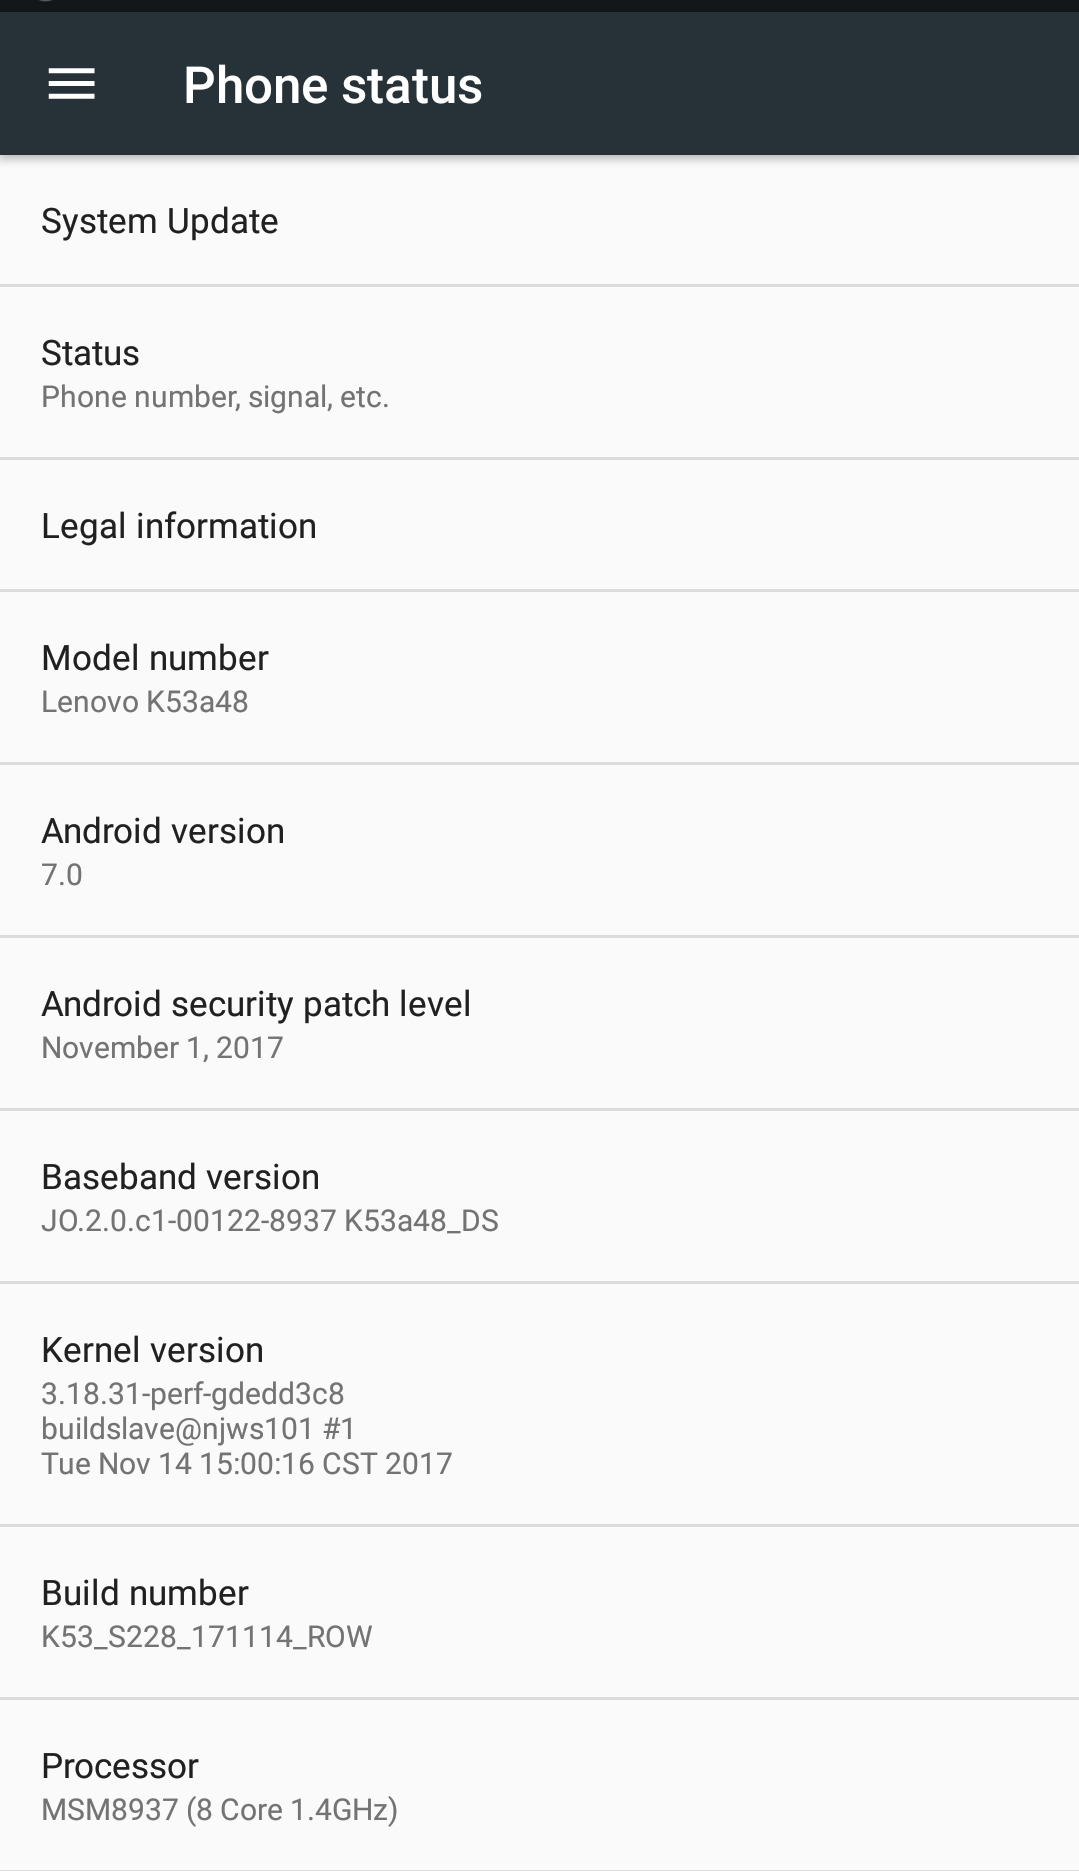
\includegraphics[width=8cm]{pictures/android_info[1].jpeg}
  \end{center}
  \caption{Android System information}
  \label{fig:android_info}
\end{figure}

\begin{figure}[H]
  \begin{center}
    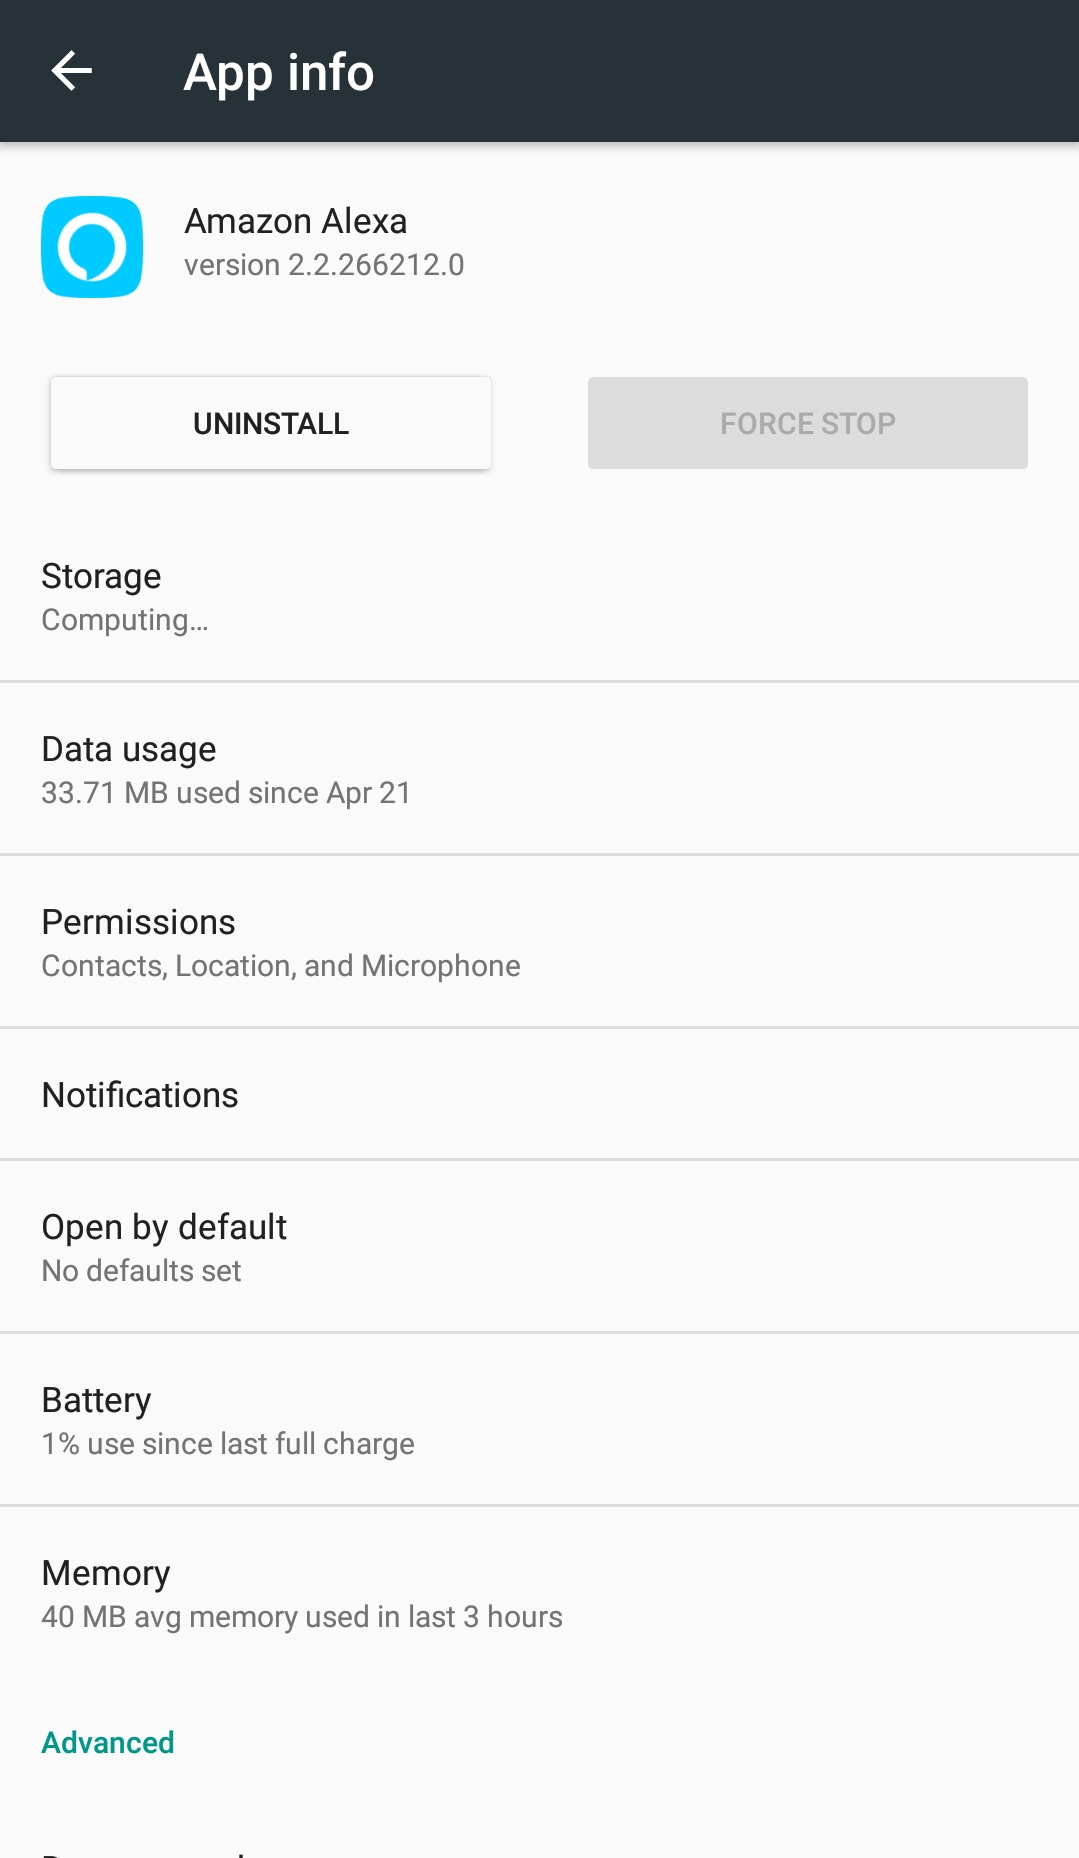
\includegraphics[width=8cm]{pictures/amazon_alexa_info[1].jpeg}
  \end{center}
  \caption{Amazon Alexa application information}
  \label{fig:alexa_app_info}
\end{figure}

\begin{table}[H]
    \begin{tabular}{ | p{6cm} | p{6cm} |}
    \hline
    QUESTION & ANSWER \\
    \hline
    Who are you? 
    & 
    I'm Alexa.
    \\
    \hline
    What's the weather in Banská Bystrica, Slovakia?
    &
    Which city in Slovakia?
    \\
    Banská Bystrica.
    &
    Sorry. I didn't get that location.
    \\
    \hline
    What is the final score of last Boston Bruins match?
    &
    Last night the Bruins beat the Maple Leafs. Four to two. They will play tomorrow at two a.m. against the Maple Leafs. 
    \\
    \hline
    How far is it from Brno to Prague?
    &
    Bruneau is 8,167 kilometres from Prague, as the crow flies.
    \\
    \hline
    Where is the Faculty of Informatics Masaryk University?
    &
    Sorry. I don't know that.
    \\
    \hline
    What is 25+25*25?
    & 
    25+25*25 is 650.
    \\
    \hline
    \end{tabular}
    \caption{Amazon Alexa - Simple questions}
    \label{tab:alexa_simple_questions}
\end{table}

\begin{table}[H]
    \begin{tabular}{ | p{6cm} | p{6cm} |} 
    \hline
    QUESTION & ANSWER \\
    \hline
    Who won the last NHL championship?
    & 
    The last winner of Stanley Cup was Washington Capitals.
    \\
    Who was the captain?
    &
    This might answer your question: Captain is the name most often given in English-speaking navies to the rank corresponding to command of the largest ships. The rank is equal to the army rank of colonel. Equivalent ranks worldwide include ``ship-of-the-line captain'', ``captain of sea and war'', ``captain at sea'' and ``captain of the first rank''. Did that answer your question?
    \\
    How tall is he?
    &
    I didn't catch that.
    \\
    \hline
    What is the capital of Russia?
    &
    The capital of Russia is Moscow.
    \\
    What is the population?
    &
    According to the US Census Bureau, the world population today is approximately 7.57 billion. 
    \\
    How far is it from Brno?
    & 
    Sorry. I don't know that.
    \\
    \hline
    Who is the Detroit Red Wings goalie?
    &
    I know about five Detroit Red Wings goaltenders. They're Jonathan Bernier, Jimmy Howard, Tom McCollum, Hari Sateri and Kaden Fulcher.
    \\
    What is his save percentage
    &
    Sorry. I don't know that.
    \\
    How old is he?
    & 
    Hawaii was admitted into the union on August 21, 1959, 60 years ago.
    \\
    \hline
    \end{tabular}
    \caption{Amazon Alexa - Conversation}
    \label{tab:alexa_conversation}
\end{table}

\begin{table}[H]
    \begin{tabular}{ | p{6cm} | p{6cm} |} 
    \hline
    QUESTION & ANSWER \\
    \hline
    Set a timer for five seconds.
    & 
    Timers are not currently supported on this device.
    \\
    \hline
    Set alarm for 7 a.m.
    &
    Alarms are not currently supported on this device.
    \\
    \hline
    Call Michaela Mravíková.
    &
    To make calls, first register in the conversations tab.
    \\
    \hline
    Play some music.
    &
    I can't find any music in your library.
    \\
    \hline
    Take a selfie.
    &
    Amazon photos is not supported on this device.
    \\
    \hline
    \end{tabular}
    \caption{Amazon Alexa - Commands}
    \label{tab:alexa_commands}
\end{table}

\section{Evaluation}

Amazon Alexa did not do very well in my tests. Problems with understanding and evaluating were visible since the first part containing only simple questions \ref{tab:alexa_simple_questions}. Amazon Alexa could not understand the names of cities I used. Therefore, two of the questions were wrong due to that problem. Amazon Alexa was able to answer one more question. Therefore Alexa gets only three points out of six for this part.

The second part was a struggle for Alexa as well. Alexa correctly answered only the first question of each triplet of conversational test questions \ref{tab:alexa_conversation}. Alexa did not understood any of the follow-up questions. As an answer to the last question from triplet of questions about Detroit Red Wings goaltenders Alexa said a fact about Hawaii for some unknown reason. I subtract one point due to that. Therefore Alexa gets only two points out of nine.

Last part of tests for Alexa is a little questionable, due to Android application having some restrictions to the use of Alexa. Nevertheless, from the answers received, and the knowledge I have on Alexa I know that all these features are supported by Amazon's assistant \ref{tab:alexa_commands}. Therefore, I give Alexa three points out of five for the last part of my tests.

Amazon Alexa scored eight points out of twenty points total.

\chapter{Google Assistant}\label{ch:google}
\section{About}

Google Assistant was first introduced as part of the Google Home smart speaker at Google's developer conference in May 2016. At first, it was just part of a chat application, and it was far from perfect. Proof of special treatment in the development of Google Assistant is that Google hired ex-Pixar animator Emma Coats to create and give the Assistant a little more personality. Google wanted to make the assistant more friendly and it has been done by giving it ``personality'', and a few funny answers. Google Assistant should behave like it had a life and people could relate to it \parencite{google_childhood}.

Before the first appearance on Android smartphones running Android 6.0 Marshmallow or Android 7.0 Nougat in February 2017, it was exclusive to Pixel and Pixel NL smartphones. After that Google Assistant slowly found its way to Android Wear 2.0, Android TVs, laptops, cars and tablets. Google Assistant was also released to iOS operating system devices as a stand-alone app in 2017 \parencite{google_ios}.

Initially, Google Assistant was operated by voice. However, user interaction with Google Assistant can be done in two ways since 2017. The other way to command Google Assistant is by typing. That approach might be useful in certain situations. For example in a loud environment when the assistant would not understand the voice command correctly. On the other hand, this is a helpful feature in a quiet environment, when the user does not want to be heard by people around him. Furthermore, this feature completely changes the behavior of the assistant giving you a reply. The reply is not spoken as usual, it is strictly visual \parencite{google_type}.

On May 08 2018 Google announced an extension to Google Assistant, called Google Duplex. Google Duplex is an AI system for conducting natural conversations. Google Duplex technology itself is not able to make general conversation without being intensely trained. The technology allows people to have as natural conversation with the machine as possible, without people having to adapt to a computer. Google Duplex technology was designed to perform tasks, such as scheduling individual appointments. For example, it can schedule a hair salon appointment, order a meal, even call a restaurant and reserve a table \parencite{google_duplex}.

\section{Privacy and Security}
Possible security and privacy risks for Google Assistant I am going to analyze are the following:
\begin{compactitem}
  \item Always Listening
  
Google Assistant as it is running on smartphones, smart home devices, and many more, supports the wake word too. For Google Assistant it can be ``Ok Google'' or ``Hey Google''. Furthermore, for voice commands to work at all, it is necessary to allow Google Assistant full access to the microphone of the device it is running on, meaning Google controls your microphone. Considering this, it is up to the user to decide whether he wants to use voice commands or not since we already know that Google Assistant can be controlled with keyboard input too. Moreover, if the user wants to use voice commands, nevertheless does not want to have the feeling of Google spying and listening all the time, Google gives an option to turn off the ``Ok Google'' function \parencite{google_turnoff}. Therefore, if the user opts for this setting, Google Assistant is still fully functional after opening the user interface.

  \item Camera
  
Google Assistant in smartphones does not ask for camera access since it is not capable of working with it. Smartphone users are still able to command their Google Assistant to ``take a picture'', although as a response the assistant only gives the list of applications capable of taking pictures and starts the selected one. Aside from that, there are plenty of cameras on the market compatible with Google Assistant and Google Home \parencite{google_camera}. These devices offer non-stop home security and surveillance. The camera is always running, connected to your Google Home, providing the video footage by streaming it to a compatible device at any time the user asks the assistant to do so. Nevertheless, some cameras are used indoors, for example, to watch over kids. Google Home, Google Assistant, cameras, everything is controlled by the software and by whom the software is controlled by. Therefore there is always the possibility of someone unwanted watching. 

  \item Discussions Are Recorded
  
Google Assistant keeps track of what the user has been asking for and all the replies given. There is a full history of these discussions with the assistant. It is easy to find, and there are multiple ways. It is possible through the Google Home and Google Assistant applications, or through the web at \href{https://myactivity.google.com/myactivity}{myactivity.google.com} \parencite{google_history}. These discussions might be private, and the user might want to keep them safe from others. Since there is the possibility, and it is easy to find and see the history, therefore any misuse of his devices can fail this wish of the user. Fortunately, in addition to easy access to history, Google gives the possibility to delete the activity log - the history \parencite{google_history2}.

  \item Susceptible to Hacking
  
Like any other software, Google Assistant and Google products are vulnerable to hacks. The real question is if these vulnerabilities are a potential risk. There is a hacker who claims, that the Google Home Hub device is at risk. The claim says: ``anyone could restart the entire Home Hub, delete the currently configured wireless network or disable notifications, such as those attached to safety devices like locks and alarms''. Hacker created a detailed post and brought up more interest in the topic. Google is aware, and it sounds like they confirm what has been said \parencite{google_hacks}.

  \item New Forms of Advertising
  
Google Assistant got popular over the years and it is installed on more than a billion devices. One of Google Assistant features is to search for anything using google. Everyone who used google already knows that the first few results are ads. Web pages or their content is related to the search query, and the owner paid Google for the advertisement. Since the advertisement is money-making for Google, they decided to prioritize advertisement results to searches done by the Google Assistant \parencite{google_ads}.

\end{compactitem}

\section{Tests}

I have tested Google Assistant on Lenovo K6 Note phone. The phone was running last available Android 7.0 software \ref{fig:android_info2}. I used Google Assistant built-in Google application running on Android software. Application was updated to the latest version 9.61.9.21.arm64 \ref{fig:google_app_info}.

\begin{figure}[H]
  \begin{center}
    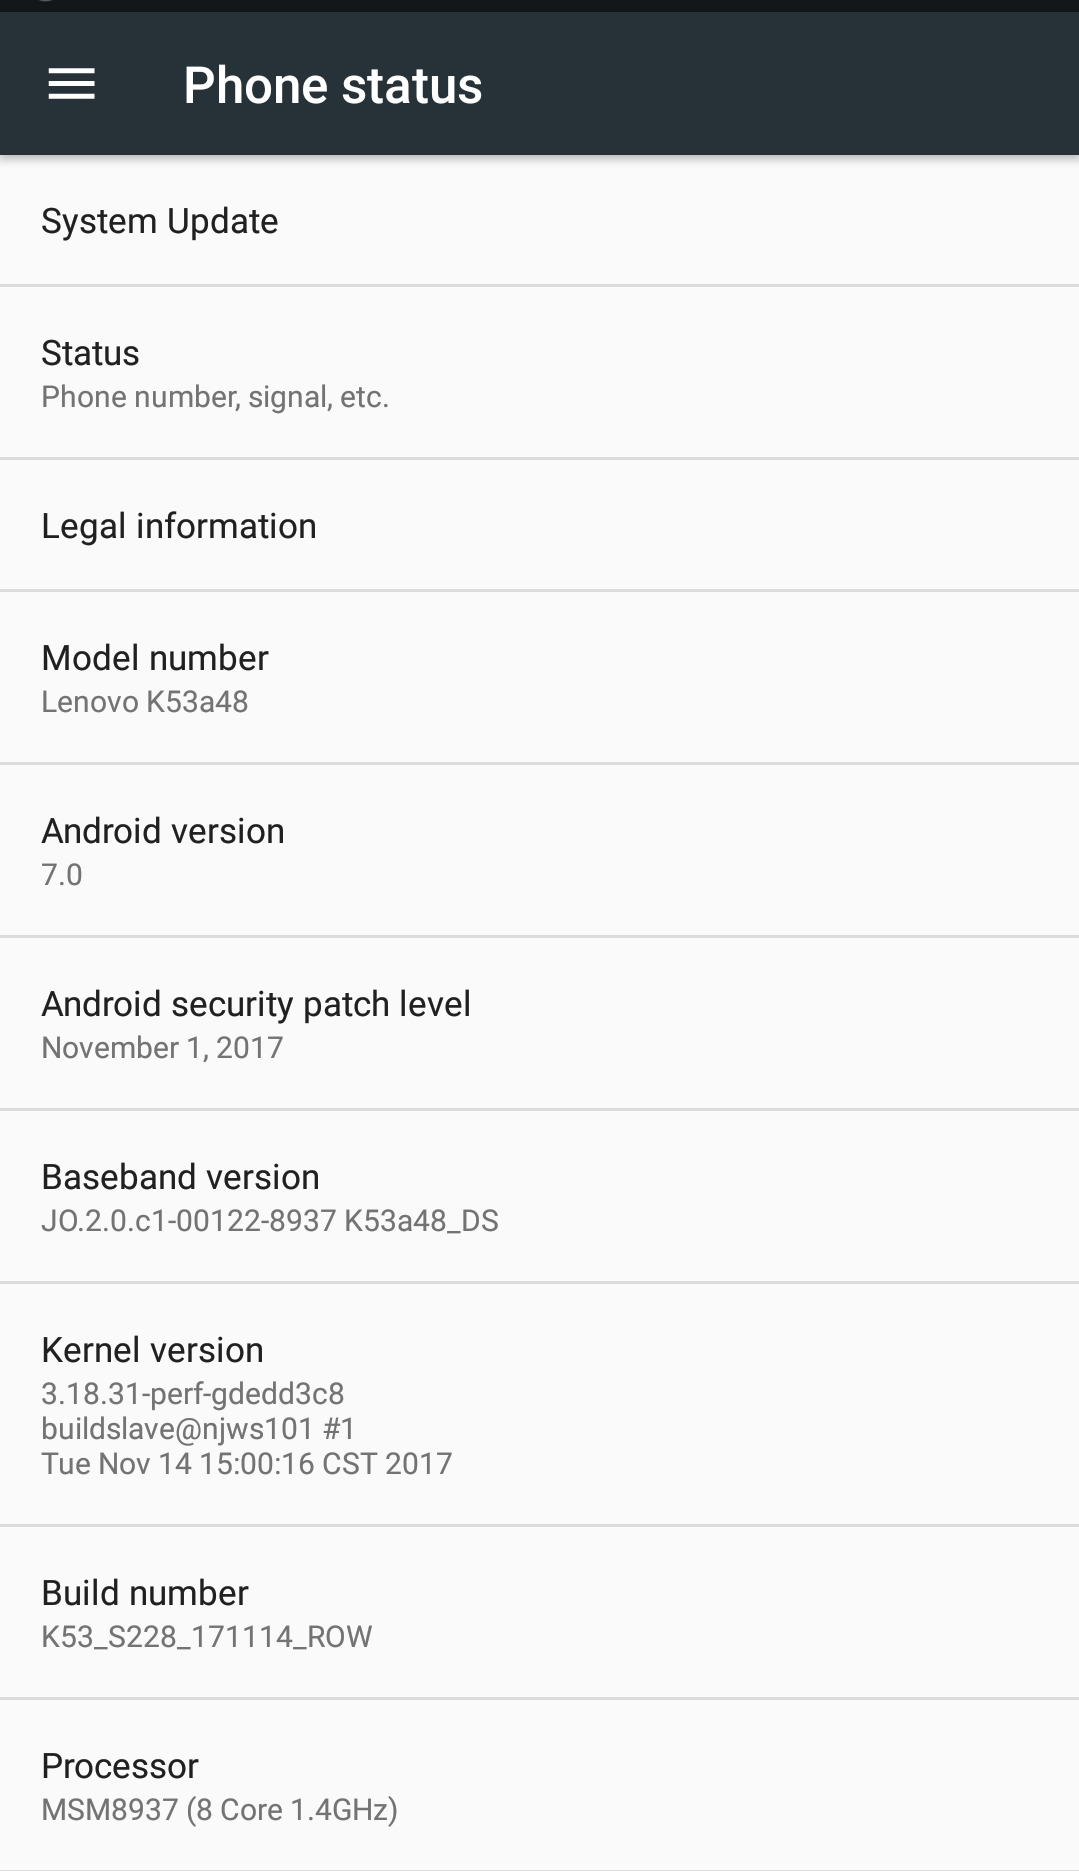
\includegraphics[width=8cm]{pictures/android_info[1].jpeg}
  \end{center}
  \caption{Android System information}
  \label{fig:android_info2}
\end{figure}

\begin{figure}[H]
  \begin{center}
    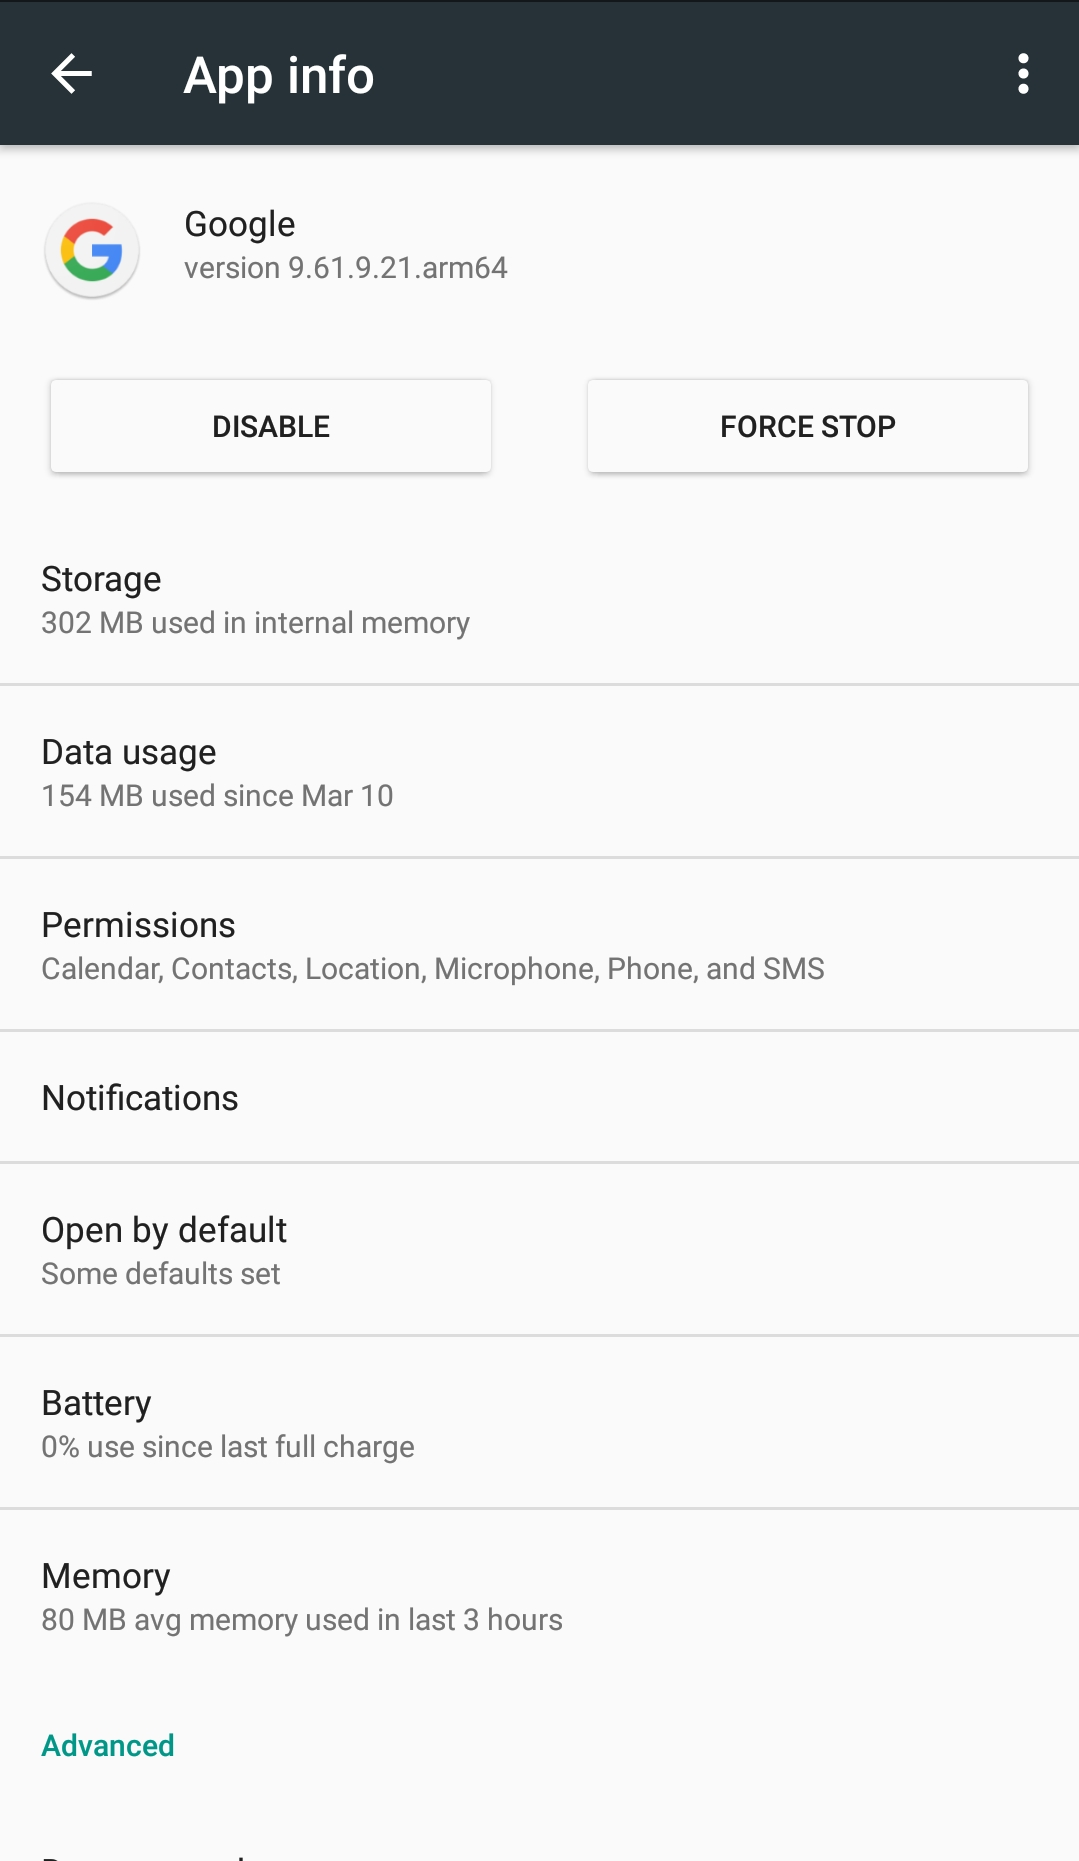
\includegraphics[width=8cm]{pictures/google_application_info[1].jpeg}
  \end{center}
  \caption{Google application information}
  \label{fig:google_app_info}
\end{figure}

\begin{table}[H]
    \begin{tabular}{ | p{6cm} | p{6cm} |}
    \hline
    QUESTION & ANSWER \\
    \hline
    Who are you? 
    & 
    I'm your Google Assistant. 
    \newline
    I can set timers for you, help you check the weather.
    \newline
    Or tell you how far Timbuktu is from here. 
    \\
    \hline
    What's the weather in Banská Bystrica, Slovakia?
    &
    Right now in Banská Bystrica it's sixteen degrees and mostly cloudy.
    \newline
    Today, there'll be scattered showers, with a forecast high of seventeen and low of seven.
    \\
    \hline
    What is the final score of last Boston Bruins match?
    &
    The Bruins won four to two yesterday against the Maple Leafs.
    \\
    \hline
    How far is it from Brno to Prague?
    &
    If you drive, Prague is two hundred six kilometers away from Brno.
    \\
    \hline
    Where is the Faculty of Informatics Masaryk University?
    &
    The address for Faculty of Informatics Masaryk University is Botanická 68A, 602 00 Brno-Královo Pole-Ponava, Czechia.
    \\
    \hline
    What is 25+25*25?
    & 
    The answer is 650.
    \\
    \hline
    \end{tabular}
    \caption{Google Assistant - Simple questions}
    \label{tab:google_simple_questions}
\end{table}

\begin{table}[H]
    \begin{tabular}{ | p{6cm} | p{6cm} |} 
    \hline
    QUESTION & ANSWER \\
    \hline
    Who won the last NHL championship?
    & 
    The NHL was won by Washington Capitals.
    \\
    Who was the captain?
    &
    Their captain is Alexander Ovechkin.
    \\
    How tall is he?
    &
    He is 1.91 meters tall.
    \\
    \hline
    What is the capital of Russia?
    &
    Moscow is the capital of Russia.
    \\
    What is the population?
    &
    The population of Moscow was 11.92 million in 2012.
    \\
    How far is it from Brno?
    & 
    Brno is 1 803 kilometres away from Moscow by car.
    \\
    \hline
    Who is the Detroit Red Wings goalie?
    &
    Jimmy Howard and Jonathan Bernier are goaltenders for the Detroit Red Wings.
    \\
    What is his save percentage
    &
    According to Detroit Free Press:
    \newline
    From the 2016-17 season through 2017-18 season, Howard accumulated a .915 save percentage and 2.63 goals against average.
    \newline
    He has been one of the Wings' best players this season, better than his .907 save percentage and 3.07 goals-against average through 47 games reflect.
    \\
    How old is he?
    & 
    He is 35 years old.
    \\
    \hline
    \end{tabular}
    \caption{Google Assistant - Conversation}
    \label{tab:google_conversation}
\end{table}

\begin{table}[H]
    \begin{tabular}{ | p{6cm} | p{6cm} |} 
    \hline
    QUESTION & ANSWER \\
    \hline
    Set a timer for five seconds.
    & 
    Okay.
    \newline
    Five seconds.
    \newline
    Starting now.
    \\
    \hline
    Set alarm for 7 a.m.
    &
    You got it. 
    \newline
    Your alarm is set tomorrow at 7 a.m.
    \\
    \hline
    Play some music.
    &
    Sure. 
    \newline
    Asking Spotify to play some music.
    \\
    \hline
    Call Michaela Mravíková.
    &
    Calling Michaela Mravíková.
    \newline
    Mobile.
    \\
    \hline
    Take a selfie.
    &
    Opening app.
    \\
    \hline
    \end{tabular}
    \caption{Google Assistant - Commands}
    \label{tab:google_commands}
\end{table}

\section{Evaluation}

The first part of the tests was straight forward \ref{tab:google_simple_questions}. Questions were not too hard and I expected Google Assistant to reply without any problem. I like the way Google Assistant is replying to question ``Who are you?'' by giving the user some hints on how to use the assistant as well. There is not much to say about this part, Google Assistant did everything right, answered every question correctly. I am giving Google Assistant five six out of six points for this part.

The second part of the tests tested the conversational skills of Google Assistant \ref{tab:google_conversation}. Three blocks with three questions each were composed to test how the assistant will understand the follow-up questions to previous answer. The Google Assistant did not have any problems answering these questions either. The answers were accurate, giving me what I asked for. I am giving Google Assistant nine out of nine points for the second part.

The last part of my tests was focused to test the assistants skills in the device usage \ref{tab:google_commands}. This part contained a few commands to see, if the assistant can be helpful in opening applications or setting timers and alarms. I was a bit disappointed with the last one "Take a selfie." Google Assistant just opened camera app, using the latest settings. Google Assistant did not take the photo, neither activated the front camera. Therefore, I give Google Assistant just four points out of five for the last part of the tests.

Google Assistant scored eighteen out of twenty points total.

\chapter{Apple Siri}\label{ch:siri}
\section{About}
Siri is a virtual assistant created by Apple Inc. and is included on all their devices with watchOS, macOS, tvOS and of course iOS operating systems. But Siri was not initially created by Apple. In the beginning, it had been an application for the iPhone developed by the 24-member startup team. Later this application was acquired by Apple for about \$200 million \parencite{siri_buy}. The startup wanted something easy to remember, short to type, comfortable to pronounce, and a not-too-common human name. As a surprise, Apple kept the original name \parencite{siri_name}.

In 2009, before Steve Jobs contacted the Siri startup, they signed a deal to make Siri a default app for all Android phones, but when Apple bought Siri they insisted on Siri being exclusive to Apple devices. After Apple acquired Siri, they updated Siri's language and expanded its linguistic range from one to multiple languages. Apple also integrated Siri into the iPhone, so it could handle dozens of Apple's tools such as task scheduling, replying to emails, checking the weather, etc.

Siri as a part of the iPhone was first introduced at a 2010 tech conference. It was able to buy tickets, register for a separate service, place a call or reserve a table, summon a taxi, all without a user having to open another app. At that time Siri had been able to connect with 42 different web services, such as Wolfram Alpha and Yelp and return a single answer that integrated the best information obtained from those sources \parencite{siri_rising}.

Currently, Siri is a part of all iPhones, Apple Watches, Apple HomePods... Since Siri is a smart virtual assistant that people buy and place in the middle of their homes, Siri's compatibility, options, and skills spread even more. Siri nowadays can control lights, thermostats, switches, outlets, windows, air conditioning and so many other smart devices the user can purchase. There is a full list of compatible devices on Apple's website \parencite{siri_compatibility}. 

\section{Privacy and Security}

To analyze Siri's privacy and security risks I will look at the following categories:

\begin{compactitem}
  \item Always Listening
  
Apple is one of the companies caring about customer privacy. As we already know, ``always listening'' is one of the privacy and security risks of any virtual assistant. Siri is always listening. However, it is not spying on users. Siri has a limited memory buffer. The buffer rewrites itself with new data constantly. This piece of audio is analyzed locally to match the trigger phrase ``Hey Siri''. Siri only wakes up and starts listening when the sample corresponds with the trigger phrase, therefore, Siri is not eavesdropping on users, and this should not be considered as a risk \parencite{siri_listening}.

  \item Discussions Are Recorded
  
It is quite reasonable to store a history of conversations with the assistant considering what we discovered about Google Assistant and Amazon Alexa regarding this problem. Apple takes a different approach when it comes to storing the data about Siri conversations. After Siri wakes up, listens to users request, Siri sends the recorded audio attached to an anonymous identification number. This identification number is not related to the user's Apple ID. There is a disadvantage to this anonymity too. The user cannot see his history older than one day. Only the most recent requests and replies are available to see typically. Furthermore, the user can change the identification number at any time \parencite{siri_recordings}.

  \item Camera
  
Camera usage is a weaker Siri point of use. Since its launch, Siri has been an iPhone feature. All iPhones have an integrated camera. Therefore Siri must have the possibility to work with it. It does, however it does not give full control. Siri can start the user's camera app, launching it with user preferred settings, or modifying the settings according to the command given. For example video, slow-motion video, selfie, and many others. Although that is nice, it is pretty much all Siri can do with the camera in iPhone \parencite{siri_camera}.
  
  \item New Forms of Advertising
  
Apple claims they are not like other companies, such as Facebook and Google. Apple argues with the fact that the user cannot be linked to their request and replies created during user-Siri conversations. Apple says it is in order to prevent target-marketing. We might not find any advertisements on Siri. However, the advertisers are smart enough, to make their TV or Radio ads to trigger the Siri on Apple HomePod devices. For example, there is an ad for the NBA which triggers Siri to inform the user about the NBA schedule.

  \item Susceptible to Hacking
  
Every software is susceptible to hacking. After all, it is just a piece of code. Apple does not cooperate with many other companies, therefore there are not many compatible devices to work with ones from Apple. Thanks to that, Apple has a more enclosed system than the other companies. It makes it harder to get enough information to bypass their systems. However, there is always someone smart enough to find a way to do so. For example, there is a programmer who found a way to display contacts through a locked screen of an iPhone when in physical possession of the phone. Siri refuses to give anything at first, however, after a series of commands Siri gives up the contact list \parencite{siri_hacking}.

\end{compactitem}

\section{Tests}

I have tested Apple Siri on iPhone XR. Operating system of the device was iOS 12.2 \ref{fig:ios_info}. Siri is integrated application of an iOS and was unable to find more information about the version.

\begin{figure}[H]
  \begin{center}
    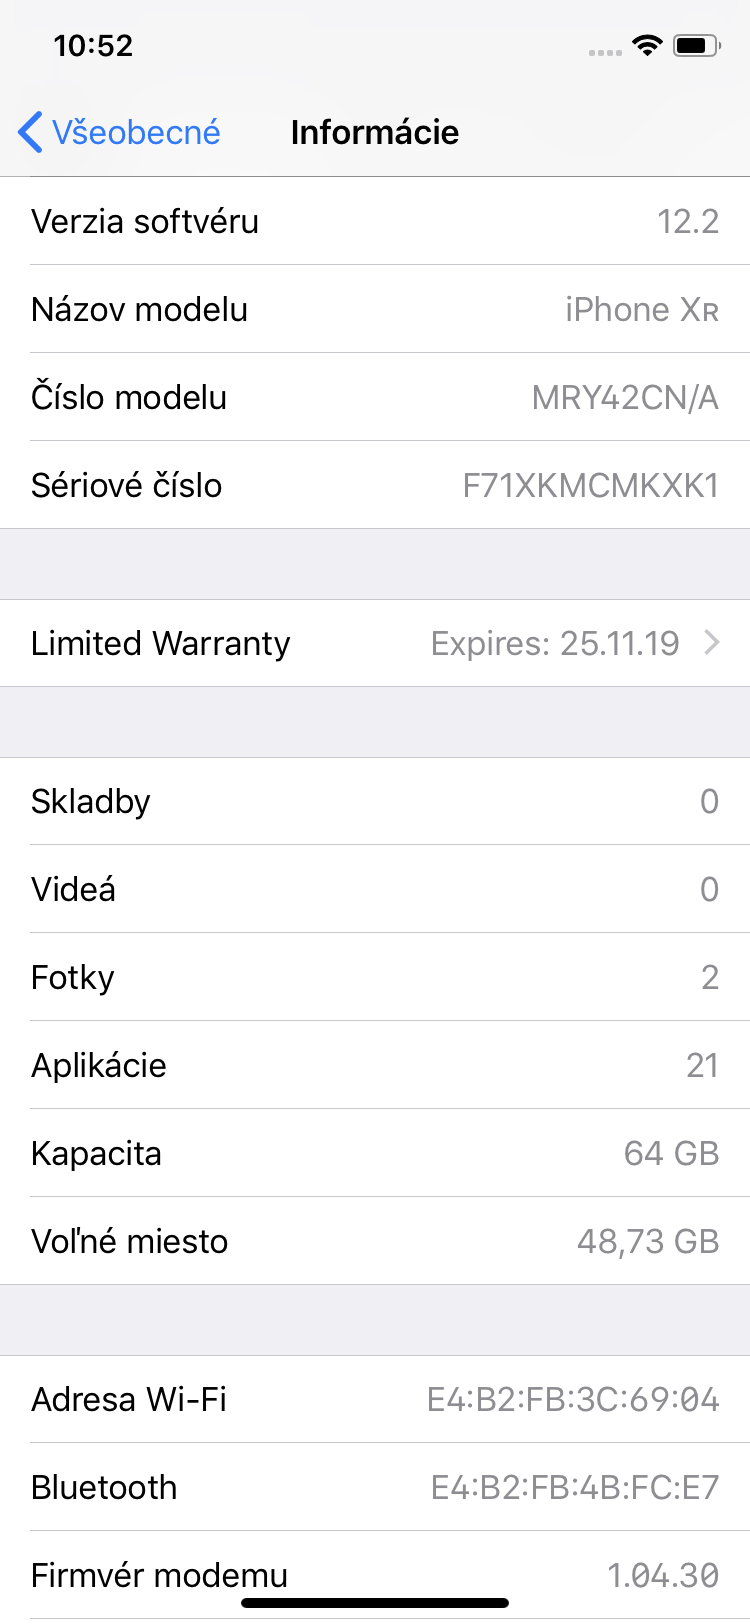
\includegraphics[width=8cm]{pictures/ios_info.PNG}
  \end{center}
  \caption{Android System information}
  \label{fig:ios_info}
\end{figure}

\begin{table}[H]
    \begin{tabular}{ | p{6cm} | p{6cm} |}
    \hline
    QUESTION & ANSWER \\
    \hline
    Who are you? 
    & 
    I'm just a humble virtual assistant.
    \\
    \hline
    What's the weather in Banská Bystrica, Slovakia?
    &
    Sorry, I can't get any information about 'Boscobel Street a Slovakia'.
    \\
    \hline
    What is the final score of last Boston Bruins match?
    &
    The Bruins beat the Maple Leafs by a score of 4 to 2 in game 6 of the first round of the playoffs yesterday. The series is now tied, 3-3.
    \\
    \hline
    How far is it from Brno to Prague?
    &
    Brno, the Czech Republic is about 193 kilometres away as the crow flies.
    \\
    \hline
    Where is the Faculty of Informatics Masaryk University?
    &
    Ok, here's what I found: \textit{(Here Siri supplied map directions to Óbuda University John von Neumann Faculty of Informatics)}.
    \\
    \hline
    What is 25+25*25?
    & 
    It's 650.
    \\
    \hline
    \end{tabular}
    \caption{Apple Siri - Simple questions}
    \label{tab:siri_simple_questions}
\end{table}

\begin{table}[H]
    \begin{tabular}{ | p{6cm} | p{6cm} |} 
    \hline
    QUESTION & ANSWER \\
    \hline
    Who won the last NHL championship?
    & 
    The Capitals won the Stanley Cup Final 4-1 over the Golden Knights. They won the last game 4 to 3 on June 8, 2018.
    \\
    Who was the captain?
    &
    Here are some results I found: Edward Smith, Abel Tasman, Francesco Schettino, Sig Hansen, Phil Harris, Don Young, Owen Chase, Günther Prien, Arne Rinnan and James S.C.Chao
    \\
    How tall is he?
    &
    Here is what I found: \textit{(Here Siri supplied a website search with resulting titles such as How tall is Captain America? - Quora, and Age of the captain - Wikipedia)}.
    \\
    \hline
    What is the capital of Russia?
    &
    Moscow is the capital of Russia.
    \\
    What is the population?
    &
    In 2017, the population of Russia was 146,804,372.
    \\
    How far is it from Brno?
    & 
    I'm sorry, I don't have any places to show.
    \\
    \hline
    Who is the Detroit Red Wings goalie?
    &
    These are the goalies for the Red Wings: \textit{(Here Siri supplied photos, numbers and names of the two Red Wings goalies: Jonathan Bernier and Jimmy Howard)}.
    \\
    What is his save percentage
    &
    Which sport? Hockey or Socker?
    \\
    Hockey.
    &
    Alright, here's what I got: \textit{(Here Siri supplied some other information about Hockey)}.
    \\
    How old is he?
    & 
    I found this on the web: \textit{(Here Siri supplied some other information about Hockey)}.
    \\
    \hline
    \end{tabular}
    \caption{Apple Siri - Conversation}
    \label{tab:siri_conversation}
\end{table}

\begin{table}[H]
    \begin{tabular}{ | p{6cm} | p{6cm} |} 
    \hline
    QUESTION & ANSWER \\
    \hline
    Set a timer for five seconds.
    & 
    Your timer is set for five seconds.
    \\
    \hline
    Set alarm for 7 a.m.
    &
    Ok, it's on.
    \\
    \hline
    Call Marko.
    &
    Which phone number for Marko? Mobile or Home?
    \\
    Home.
    &
    Calling Marko - home...
    \\
    \hline
    Play some music.
    &
    Beats 1 coming right up... \textit{Siri playing internet radio}.
    \\
    \hline
    Take a selfie.
    &
    \textit{Siri opens camera application and switches to front camera}.
    \\
    \hline
    \end{tabular}
    \caption{Apple Siri - Commands}
    \label{tab:siri_commands}
\end{table}

\section{Evaluation}

I encountered issues with Siri immediately at the start of testing in the first part of the tests \ref{tab:siri_simple_questions}. Siri has troubles understanding names (of places) that include diacritics, such as ``Banská Bystrica''. Another misunderstanding was with word ``Masaryk''. Siri did not understood, therefore Siri gave me a wrong answer. I tried the same question a few time of record, but even with correct understanding of word ``Masaryk'' I was given the same wrong answer. Therefore, Siri gets four out of six points for this part.

The second part showed more problems. Siri gave good answers only for three and a half out of 9 questions \ref{tab:siri_conversation}. Siri was not able to follow-up the questions. Siri did not understand continuous conversation, and did not identify the subject correctly. There was only one partially correct answer on the follow-up question. After asking for the capital of Russia, I wanted to know the population of Moscow, but Siri gave me population of Russia. I count this as a partially correct answer, because it might not be straight forward if I am asking for population of Russia or Moscow. I give Siri three point five points out of nine for the second part.

In the last part, Siri did well as I expected. Without any problems performed all the commands it was given \ref{tab:siri_commands}. There was only one weak action. When I asked Siri to take a selfie, she opened the camera application and switched to front camera. Eventually, Siri never took the picture. Therefore I give Siri four point five out of five points.

Siri scored twelve out of twenty points total.

\chapter{Comparison}

Based on the research I made on the topic of the virtual assistants, especially on Amazon Alexa, Google Assistant and Apple Siri and the tests I have performed, I can say that that Google has done the best job in the development. I am not sure about what to think about Apple's Siri. I expected a lot more from Apple and their implementation. I do not think Siri is part of the most evolved and smart assistants available on the market. Alexa seems like an average assistant to me. It is available to anyone, because it is not as expensive as Apple's devices with Siri and Alexa looks to be capable of working with the most other devices, such as smart lightbulbs, and valves...

Google Assistant scored eighteen points in my tests and that is the highest score. That explains everything I would say. Google Assistant seems to understand pretty much anything and gives relevant and correct answers. It is the only assistant, from those I tested, that supports written input too. I find helpful and nice, that Google Assistant writes on screen what it hears in real time, some do not do it at the end with the reply, some do not do it at all. I haven't used any of the assistants before. The experience I have now, after preparation of this thesis, I can say that Google Assistant is the one most pleasant and comfortable.

I will put Amazon Alexa to the second place, even though Alexa scored only eight points. Alexa might not be as ``smart'' as Google Assistant, but for a standard user, who does not require the smartest assistant that will be chatting with him during late evenings and discuss the worlds hardest problems it is sufficient. Also, Alexa is capable to communicate and command many smart home appliances and devices and I think this number is higher than Siri's and Google Assistant's. Alexa is not expensive either. Amazon's Alexa and the Amazon Echo devices are one of the most affordable devices on the market.

Apple's Siri on the other hand, is definitely the most expensive one. It does not matter if we look at the Apple HomePod or iPhones, these are the ones of the most expensives devices of their kind. After what I have experienced with Siri, I do not think it is worth the money. To be honest, Siri is an average assistant and even might be below the average, there is a lot of them out there that I have not tested. I expected Siri to understand more, not to have problem with different accents, and non-English city names. Apple and their Siri disappointed me.

I am not the only one who tested virtual assistants. Marques Brownlee made a video of his tests on his youtube channel \parencite{brownlee_battle}. Even though the video is from 2017 it is still accurate in my opinion. He tested Google Assistant, Amazon Alexa, Samsung Bixby, and Apple Siri. The conclusion was: Google Assistant did what he asked for, did not have problems answering his questions; Apple Siri got the job done, sometimes Siri replied in a strange way; Samsung Bixby was not bad, although it was not replying in natural human style and it sounded robotic; Amazon Alexa was the worst one.

Andy Wood and Matt Kirshen tested understanding of various accents on Amazon Alexa, Google Assistant, and Apple Siri in their video for the channel \textit{WIRED} \parencite{wired_accents}. In their video we can see eight people with different accents asking the assistants the same thing. The result was clear. Google Assistant was the best one of the three mentioned to understand the most of the used accents. Apple Siri ended up second followed by Amazon Alexa in the third place.

\chapter{Perfect virtual assistant design}

\section{Being offline}
After testing Google Assistant, Apple Siri, and Amazon Alexa and analyzing their flaws, privacy and security risks I will say the most important characteristic of perfect assistant would be ``being OFFLINE''. It is unrealistic for the current era. 

It would be too expensive to put the required computing power into single device which would make the device unaffordable for the consumers to buy the product. That computing power is necessary for virtual assistant to run fast and smoothly. Therefore all of the actual assistants are running on clouds. 

The assistant is not only using internet to communicate with the cloud computers for the speech recognition and using evaluation of the user's command. The internet connection is used to search for the results on the web, to search the definitions... Therefore it will not be possible for an assistant with features depending on internet connection to be completely offline, at least not until the single device will be capable of storing all of the information on the internet and constantly updating, which is unlikely to happen.

Furthermore, having the assistant entirely run on a customer's device could be a potential risk for the manufacturer. The technology and know-how for software like virtual assistant is expensive to develop, therefore the developers want to keep it safe. If the assistant is running on customers device customer could try to decompile the assistant, analyze the code and steal the technology.

\section{Listening notification}
Another key feature should be a notification that a microphone or a camera is being used in the background. By that I mean using for example a LED diode to notify the user something is being used or putting a notification in the status bar of a smartphone or other device with screen the assistant will be running on. Therefore the user would be able to keep track of what the assistant is doing and he could make sure it is listening/recording only when it is supposed to.

\section{No history}
Further, I would remove the history. I do not think it is necessary for the user to see the answers to old questions. If the user forget the answer or wants to hear/read it another time he can ask the same question again. As a result of history not being stored there is no potential privacy risk that someone unwanted will read the conversation between the user and his assistant.

\section{More features and compatible devices}
In the future it will be mandatory for a virtual assistant to communicate with as many devices as possible. People will be using the assistant on daily basis. Virtual assistants will become part of human lives and it might be life changing technology that will bring us smarter, easier, and a better future.

\chapter{My implementation}


\printbibliography[heading=bibintoc] %% Print the bibliography.


\appendix %% Start the appendices.

\chapter{An appendix}
Here you can insert the appendices of your thesis.

\end{document}
